\documentclass[a4paper,12pt]{book}

\usepackage{apacite}
\usepackage{quotchap}
\usepackage{amssymb}
\usepackage{pdfpages}
\usepackage{pseudocode}
\usepackage{geometry}
\usepackage[english]{babel}
\usepackage{lscape}
\usepackage{graphicx}
\usepackage{appendix}
\usepackage{url}
\usepackage{framed}
\usepackage[framed]{ntheorem}
\usepackage{verbatim}
\usepackage{stmaryrd}
\usepackage{array}
\usepackage{caption}
\usepackage{subcaption}
\usepackage{vub}
\usepackage[T1]{fontenc}
\usepackage[scaled]{uarial}
\usepackage{tocloft}
%\renewcommand{\familydefault}{\sfdefault}
\usepackage{blindtext}
\usepackage{listings}
\usepackage{fancyhdr}
\usepackage{natbib}
\definecolor{java}{RGB}{127,0,85}
\newcommand{\code}[1]{\texttt{#1}}
\lstset{language=Java, basicstyle=\scriptsize,breaklines=true, keywordstyle=\color{java},tabsize=1, frame=single}
\newcolumntype{C}[1]{>{\centering\let\newline\\\arraybackslash\hspace{0pt}}m{#1}}
\newcolumntype{L}[1]{>{\raggedright\let\newline\\\arraybackslash\hspace{0pt}}m{#1}}
\addtocontents{toc}{\cftpagenumbersoff{chapter}}
\newtheorem{hyp}{Hypothesis} 
\newframedtheorem{defshad}{Definition}
\newtheorem{defPim}{Definition}
\newframedtheorem{pilePrinc}{Principle}
\newframedtheorem{theo}{}
\newtheorem{req}{Requirement}
\setlength{\marginparwidth}{0pt}
\makeatletter
\renewcommand*{\sectfont}{\bfseries}
\renewcommand*{\chapnumfont}{%
  \usefont{T1}{\@defaultcnfont}{b}{n}\fontsize{120}{150}\selectfont% Default: 100/130
  \color{chaptergrey}%
}
\makeatother
\geometry{textwidth=390pt}

\geometry{bindingoffset=2cm}


\fancypagestyle{plain}{
  \fancyhf{}
  \fancyfoot[C]{}%
  \renewcommand{\headrulewidth}{0pt}% Line at the header invisible
}

\makeatletter
\renewcommand\paragraph{%
   \@startsection{paragraph}{4}{0mm}%
      {-\baselineskip}%
      {.5\baselineskip}%
      {\normalfont\normalsize\bfseries}}
\makeatother

\author{Alexander Moerman}
\title{Projection of Reactive Programs onto Dataflow Engines}
\promotortitle{Promoter}
\promotor{Prof. Dr. Wolfgang De Meuter}
\advisortitle{Advisor}                                                            
\advisors{Mathijs Saey, Florian Myter and Thierry Renaux}
\faculty{Faculty of Science and Bio-engineering Sciences}
\department{Department of Computer Science}   
\subtitle{Master thesis submitted in partial fulfillment of the requirements for the degree of \\Master of Science in Applied Sciences and Engineering: Applied Computer Science}
\date{Academic year 2016-2017}
          
\begin{document}
\pagestyle{fancy}
\setlength{\headheight}{14.5pt}
\renewcommand{\chaptermark}[1]{\markboth{\MakeUppercase{\chaptername}\ \thechapter.\ #1}{}}
\renewcommand{\sectionmark}[1]{\markright{#1}{}}
\fancyhf{}
\fancyhead[LO,RE]{\bfseries\thepage}
\fancyhead[RO]{\bfseries\leftmark}
\fancyhead[LE]{\bfseries\rightmark}
\renewcommand{\headrulewidth}{0.5pt}
% PARAGRAPH INDENTATION

%\setlength{\parskip}{0pt} % 1ex plus 0.5ex minus 0.2ex}
%\setlength{\parindent}{0pt}

%\maketitlepage
\maketheses
\pagebreak
\setcounter{page}{1}
 \pagenumbering{roman}

\section*{Abstract}


            
\newpage
% !TeX spellcheck = nl_NL
\section*{Samenvatting}

Programma's in domeinen zoals robotica, het web en mobiele applicaties worden allemaal aangedreven door events. Dit inherent asynchrone model conflicteert met de synchrone aard van imperatief, sequentieel programmeren, en hierdoor zijn andere paradigma's verschenen om deze problemen beter aan te pakken. Een dergelijk paradigma dat speciaal ontworpen is voor \textit{event-driven} omgevingen is reactief programmeren, die events concretiseert als tijdvariabele waarden en ze samenstelbaar maakt aan de hand van declaratieve operatoren. Reactief programmeren probeert de uitdagingen van asynchroniciteit aan te pakken, zoals bijvoorbeeld de toepasselijk genaamde \textit{callback hell}, door een uniforme interface te voorzien voor verschillende asynchrone bronnen (e.g. I/O, events, ...) en op die manier te stroomlijnen hoe data doorgegeven wordt doorheen deze programma's.

Met dit hoge niveau van abstractie komt echter ook een bedenking met betrekking tot efficiëntie en timing, die van essentieel belang zijn voor deze systemen. Het merendeel van reactieve programma's tot nu toe zijn single threaded en benutten niet het volledige potentieel van hun onderliggende systemen. Onderzoek is reeds uitgevoerd om deze programma's te parallelliseren, maar wij stellen een ander alternatief voor: het mappen van reactieve programma's naar het dataflow executiemodel. Dit low level platform bepaalt dat primitieve instructies kunnen worden opgeroepen wanneer hun inputs aanwezig zijn, op voorwaarde dat ze geen gedeelde state uitlezen of muteren. Hierdoor kunnen niet-gerelateerde instructies (d.w.z. die geen data afhankelijkheden delen) parallel worden uitgevoerd.

In deze paper beschrijven we het proces van de vertaalslag van reactieve tijdsvariabele waarden naar instructies in het dataflow executiemodel. We presenteren twee interpreters voor een kleine experimentele taal speciaal ontworpen voor dit onderzoek: een eerste die reactiviteit in een eerder traditionele zin implementeert en een tweede die bovenop een dataflow engine draait. Daarnaast geven we een samenvatting van de mismatch tussen de twee modellen en bespreken we oplossingen hiervoor.

Tenslotte evalueren we de prestatie van beide benaderingen op vlak van efficiëntie en bespreken we de schaalbaarheid van reactieve programma's bovenop een dataflow engine. 
\newpage
\section*{Declaration of Originality}
I hereby declare that this thesis was entirely my own work and that any additional sources of information have been duly cited.
I certify that, to the best of my knowledge, my thesis does not infringe upon anyone's copyright nor violate any proprietary rights and that any ideas, techniques, quotations, or any other material from the work of other people included in my thesis, published or otherwise, are fully acknowledged in accordance with the standard referencing practices. Furthermore, to the extent that I have included copyrighted material, I certify that I have obtained a written permission from the copyright owner(s) to include such material(s) in my thesis and have included copies of such copyright clearances to my appendix. 
 
I declare that this thesis has not been submitted for a higher degree to any other University or Institution.

\newpage
\section*{Acknowledgements}

\newpage
 
\tableofcontents
\newpage
\listoffigures
\newpage
\listoftables
\newpage
\setcounter{page}{1}
 \pagenumbering{arabic}

\chapter{Introduction}

Reactive programming is becoming increasingly popular. Over the past decade, we have observed a slow but steady shift away from traditional imperative paradigms towards other, more declarative ones.
The technology landscape is moving, and with it the software development world. Web and mobile applications, the \textit{internet of things} and now virtual reality software are dominating the conversation, and they all have one thing in common: they are driven by events. Events, callbacks and asynchronous computation have always been challenging. Since callbacks are inherently not composable and do not provide a unified interface, one quickly arrives at deeply nested callbacks to perform any meaningful task, these nested structures are colloquially known as \textit{callback hell}. Furthermore, propagating and eventually surfacing errors requires manual wiring of these errors up the call chain, resulting in repetitive and difficult to maintain code. 

Reactive programming solves these problems by putting events at the forefront as first class citizens under one unified interface, reifying them as time varying values and making them composable using declarative operators. It provides a single interface over I/O, events and any asynchronous computation, switching the mindset from state through imperative modifications to state distilled from declarative derivations of events. 

\section{Problem statement}

Timing and efficiency is critical and desired for reactive systems (e.g. user interfaces, robotics, etc.).
Thus far the majority of reactive programming implementations have been single threaded and don't utilise the maximum potential of their underlying host. Slowly but surely there are parallel approaches popping up which focus on thread based or actor based concurrency \cite{peterson_parallel_2000}, but none have tried mapping these reactive programs onto something that was designed to run parallel from the beginning: the dataflow execution model. This execution model allows instruction invocation whenever the inputs are available (contrary to the sequential models such as the Von Neumann model where instructions are executed one after another) and does not have global state, which allows it to exploit all of the available parallelism in a given input program.

Reactive programming nor the dataflow execution model are new technologies, both go back to at least the 1980s \cite{harel_development_1985, veen_dataflow_1986}. While they try to solve different problems, they do share an interesting common trait: the evaluation models of both use directed graphs to orchestrate data flowing through its applications. 

The core principle of reactive programming is making events first class citizens, called signals: they can be listened to, transformed or even composed with other signals, ultimately building a graph of nodes that represent these signals and the data dependencies between them. When the application executes, data courses through this graph via the \textit{reactions} of the nodes when a signal is fired. One could say that the system \textit{reacts} to every signal.

The dataflow execution model on the other hand has a different purpose: parallelizing primitive instructions as much as possible by tracking the flow of data through them and invoking instructions as soon as their inputs are present. Unrelated instructions, which are not dependent on common data, can be executed in parallel, while related instructions are only invoked when their data dependencies are satisfied. These dependencies between instructions again form a graph. This time however, nodes in the graph represent instructions, not signals. Dependencies in this graph simply indicate that one instruction takes as input the output of another. 

So while reactive programming uses a graph of nodes which represent signals, the dataflow execution model has a graph which represents instructions. When executed, data flows through these graphs and the output of a node is forwarded to nodes further down the graph. Conceptually, nodes in these graphs mean different things in the two models, but the way that they behave is undeniably similar.

The goal of this thesis is to explore the possible benefits of running a reactive language on top of a dataflow engine, more specifically the advantages with regards to parallel execution. We propose that the update mechanism necessary to support a reactive language can be completely implemented on top of a dataflow engine, with the aim to parallelize the updating of separate nodes in the reactive graph. 
This would allow us to scale a reactive program horizontally, exploiting the maximum amount of parallelism possible. The purpose of this thesis is therefore to investigate the parallelization of reactive programs by using the dataflow execution model as a platform.

\section{Contributions}

In order to test our hypothesis, we present a new reactive programming language \textit{FrDataFlow}, based on Racket with a few extra features to natively support reactive programming. Expressions in this language are evaluated by our own interpreter, which builds the aforementioned graph in the background and keeps it up to date. Rather than implementing our own update mechanism however, the reactive graph is translated to instructions in a dataflow engine implementation as described in \textit{An Extensible Virtual Machine Design for the Execution of High-level Languages on Tagged-token Dataflow Machines} \cite{saey_extensible_2017}. This is the core mechanism that will orchestrate the events and keep nodes in the graph up to date.

Furthermore, we evaluate this approach by comparing it to an implementation of the same language that does not run on a dataflow engine, but applies a more traditional evaluation model, as described in FrTime \cite{cooper_embedding_2006}. Benchmarks are provided for both latency and throughput for both implementations. Lastly, we also investigate the scaling possibilities of FrDataFlow by actually running it across multiple cores simultaneously. 

\section{Structure}

This dissertation is structured to provide the reader with sufficient context before the actual research and evaluation is discussed. To this end, chapter 2 provides a general background with regards to both reactive programming and the dataflow execution model. It succinctly covers the problems they want to solve, how they attempt to do so, the advantages of these approaches and a short example illustrating how they work.

In chapter 3, our custom language FrDataFlow is presented, with an elaborate sample program displaying most of the features supported by the language. The evaluation of this example by our interpreter is then visually detailed with diagrams and corresponding explanations. 

The dataflow engine is discussed in chapter 4. This is an implementation of the dataflow execution model that powers the update mechanism in FrDataFlow. A short sample is provided to show how instructions are invoked in this engine, and how output from one instruction gets forwarded to the input argument of another. Next, the main research topic of this dissertation is presented: the mapping algorithm. This is the translation we make from the graph in reactive programming to a new graph of instructions for the dataflow engine. Encountered obstacles and corresponding workarounds are discussed.

Chapter 5 details the evaluation of our research. 
% TODO
*** TODO ***
*** TODO ***
*** TODO ***
*** TODO ***
*** TODO ***
*** TODO ***
*** TODO ***

In chapter 6, we summarize the boundaries at which this research has drawn a line and discuss possible future improvements or extensions to our system. We do this by recognizing features provided in other reactive languages or frameworks, that are not present in FrDataFlow. 

Related research topics are discussed in chapter 7. We took great inspiration from ambitious works such as Elm and FrTime, which we compare with FrDataFlow in terms of design and evaluation. 

Finally, we conclude with chapter 8, which summarizes our findings of this research.
*** TODO ***
*** TODO ***
*** TODO ***
*** TODO ***
*** TODO ***
*** TODO ***
*** TODO ***

\chapter{Background}

\section{Introduction}

This research builds on two existing paradigms in software development: reactive programming and the dataflow model. While intimate knowledge about these concepts is not required, a basic understanding of both will be necessary to follow the ideas and implementation of this dissertation. Reactive Programming is situated in the category of higher level software development, serving as an abstraction tool for events and reactions to those events. The dataflow model on the other hand can be considered more 'low level', providing a strategy for the implicitly parallel execution of programs. 

\newpage

\section{Reactive Programming}

Reactive Programming is a software development paradigm focused on reactions, i.e. the handling of external events, user interactions, etc.  In this paradigm, the application state is derived from the previous state and any events that may occur, for example user interactions or current environmental factors. This deviates from more traditional approaches, where values and state can be written at any point and for any reason. In a reactive program however, the flow of dependencies is recorded as a (possibly cyclic!) directed graph, making the derivation of the application state very explicit.
At the core of reactive programming are the following main concepts:
\begin{itemize}
	\item The first-class reification of events (making events a first-class citizen)
	\item The composition of these events through lifted functions
	\item The automatic tracking of dependencies and re-evaluation by the language runtime
\end{itemize}

A number of implementations exist for reactive programming, in this thesis we will focus on the interpretation taken in FrTime \citep{cooper_embedding_2006}.

\subsection{Example}

The canonical metaphor for Reactive Programming is spreadsheets, which typically track changes across input cells and automatically recompute values in other cells if the formulas they contain reference the aforementioned input cells. In essence, cells react to modifications made in other cells if their formulas depend on them. These cells are what we call \textit{observables} or \textit{signals} in Reactive Programming.
Imagine a simple program in an imperative programming setting, as shown in listing \ref{lst:background-reactive-example}.

\begin{lstlisting}[caption={A basic reactive program},captionpos=b,label={lst:background-reactive-example}]
	a = b + c
\end{lstlisting}

When this statement is executed, it assigns the result of adding b and c to the variable a, mutating a in the current scope. Note that this only happens once. A snapshot is taken of the current value of b and c, to determine the new value of variable a. Of course, this assumes that the variable b and c are provided to the program.

\begin{figure}[h]
	\centering{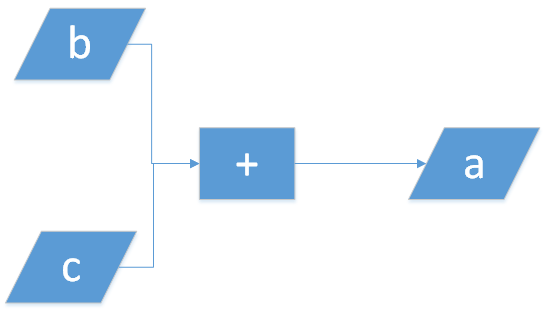
\includegraphics[width=\textwidth]{images/background-reactive-example.png}}
	\caption{Graph of signals}
	\label{fig:background-reactive-example}
\end{figure}

In a reactive programming setting, a would subscribe to the values of b and c, essentially asking to be notified whenever the variables b or c change, at which point the value of variable a changes. See figure \ref{fig:background-reactive-example} for the reactive graph. This process repeats every time the variables b or c are modified. Note that the value of a is undetermined until both b and c produce a value. 

The implementation of this reactive mechanism can be provided by the language itself or by a framework or library. 

\subsection{Advantages of Reactive Programming}

A signal can be described as "values over time", in contrast with a variable which only holds its latest value, revealing no information about the time that value was provided or what changed it. 
Signals can be used to model almost any concept in software development:
\begin{itemize}
	\item mouse movements as a signal which emits the current position in real time
	\item click events as a signal which emits event objects
	\item the results of a database query as a signal which emits only one value
    \item an infinite sequence as a signal which never stops emitting
\end{itemize}

Even though the underlying mechanism will still be identical to more traditional approaches (attaching event listeners to DOM events in HTML, opening and connecting to a WebSocket connection, etc.), the fact that all these concepts can be brought together under a single umbrella called \textit{signals} allows for the modeling of higher order operators to map, combine and filter these flows of values in ways that were previously a lot harder.

\section{The Dataflow Model}

\subsection{Introduction}

The dataflow model \citep{johnston_advances_2004} is a paradigm focused on the parallel execution of programs. In this paradigm, instructions are seen as isolated units, which should be able to execute whenever the necessary parameters have been provided. Contrary to imperative programming, instructions are not invoked by a program counter, but rather whenever all of the parameters are present. 

The execution of instructions in the dataflow model can be seen as a direct graph of nodes where each node represents an instruction and each edge is the output being sent to the next instructions that require the output as arguments. It is up to the dataflow engine to orchestrate the flow of arguments so that instructions are invoked correctly and in the correct order.

Whenever an instruction is invoked, the output is sent through to all connected instructions which depend on it. In Tagged Token Dataflow systems \citep{arvind_executing_1990}, instruction arguments are wrapped in tokens, which carry meta data about which execution context they belong to in order to isolate multiple calls to the same instruction from one another.

A large difference with Reactive Programming is that Dataflow Programming puts the instruction invocation at the center stage, while Reactive Programming puts forward signals as the core concept of its paradigm. In other words, while both systems have the notion of a dependency graph, the nodes in their graphs carry different concepts: instructions and signals respectively.
 
\newpage

\subsection{Example}

Imagine a simple program in an imperative programming setting, as shown in listing \ref{lst:background-reactive-example}.

\begin{lstlisting}[caption={A basic data flow program},captionpos=b,label={lst:background-dataflow-example}]
a = b + c
d = a + b
\end{lstlisting}

This assumes that the variable b and c are provided to the program.
In a traditional execution, the variable a would be set to the sum of b and c and the variable d would be set to the sum of a and b. Note that the sequence in which these operations are executed is of vital importance: switching the two statements would result in different values for the variable d!

\begin{figure}[ht]
    \centerline{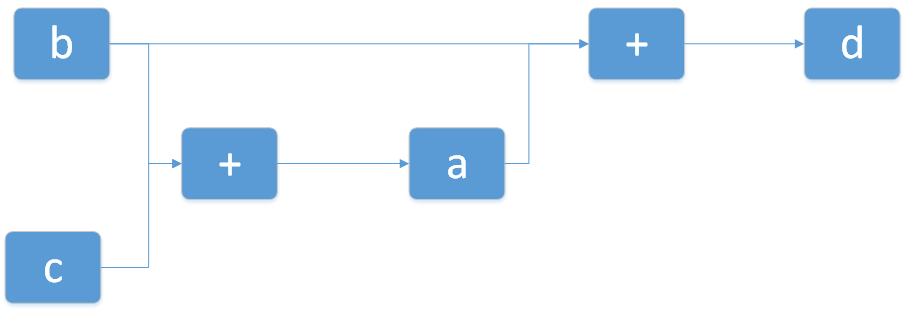
\includegraphics[width=\textwidth]{images/background-dataflow-example.png}}
	\caption{Graph of instructions}
	\label{fig:background-dataflow-example}
\end{figure}

In a dataflow engine, these instructions would be registered as instructions in the dependency graph, as visualized by figure \ref{fig:background-dataflow-example}. The values of b and c would be added to the queue at application startup. B would be entered as a token twice; once for the instruction "+" which computes a and once for the instruction "+" which computes d. When the dataflow engine spins up and starts processing arguments, it sends the tokens for b and c to the first "+" instruction, which is triggered because all of its inputs are present and valid. This produces a value for variable a, which gets added to the token queue again as the first parameter for the second "+" instruction. This instruction now also has all of its inputs present, which allows it to compute the value for variable d at this point.

If at any point in the future, b or c (which should be seen as the output of other instructions not shown in the sample code) produce new values, these would be enqueued again for further processing.

\subsection{Advantages}

The key advantage of the data flow model is that only the data dependencies of the instructions decide when an instruction can be executed. Since data flow instructions are not allowed to access or manipulate shared state, each instruction is completely isolated. This means that all dataflow instructions can be run in parallel, across different processes and even separate machines.

\section{Conclusion}

Two paradigms were presented: reactive programming and the dataflow model. 
Reactive programming is targeted more towards events and reactions and shines best in environments where these things are plenty, for example in user interfaces and other places where events can come from any direction. The dataflow model on its part focuses more on the parallel execution of instructions by streaming parameters to them in isolated scopes. We do however note similarities between the two, namely that they both work with an update graph that guides the data along the nodes. 



 
\chapter{Language}
\lstset{language=lisp,showtabs=false}

\section{Introduction}

For the purposes of this thesis, we have implemented a lightweight language called \textit{FrDataFlow} using two different AST interpreters in Racket, supporting most of the basic constructs found in Racket. This language is based on earlier work detailed in \citet{abelson_structure_1999}. The first interpreter supports reactive patterns on top of the already existing Racket language. The second interpreter also supports the exact same language, but executes its instructions using an underlying dataflow engine. We chose to implement this custom language \textit{FrDataFlow} (rather than a framework or library) to maintain maximum control over the inner workings and to facilitate experimentation atop the dataflow engine. The main goal was to have a reactive superset of Racket for experimental purposes during this thesis.

\newpage
\section{FrDataFlow}


\subsection{Sample program}

FrDataFlow provides an environment with most Racket language constructs (defining variables, procedures, lambda, primitive operators, ...), the \textit{lift} operator (which creates a new signal based on other signals) and some built in signals, shown in listing \ref{lst:language-frdataflow-builtinsignals}

\begin{lstlisting}[caption={Built in signals},captionpos=b,label={lst:language-frdataflow-builtinsignals}]
;; A signal which emits the current seconds since 1 Jan 1970, every second
current-unix-timestamp	
;; A signal which emits the current temperature from time to time
current-temp-fahrenheit 
\end{lstlisting}

Take for example a roadside digital billboard which displays the current date and temperature. To show this information, we can derive a signal that contains the exact information that needs to be shown, using the built in signals in FrDataFlow. 
From the \textit{current-unix-timestamp} signal, we can compute the date using the built in procedures \textit{seconds->date} and \textit{date->string}. The temperature is unfortunately in fahrenheit, so we will convert it to Celsius first. Lastly, we combine these signals into a single signal that contains the text we want to show. See listing \ref{lst:language-frdataflow-billboard} for the full definition of the billboard text written with FrDataFlow constructs. 

\begin{lstlisting}[caption={Billboard},captionpos=b,label={lst:language-frdataflow-billboard},mathescape,language=FrDataFlow]
(define (fahrenheit->celsius fahrenheit)
  (quotient (* (- fahrenheit 32) 5) 9))
(define current-temp-celsius
  (lift fahrenheit->celsius current-temp-fahrenheit))
(define current-date
  (lift seconds->date current-unix-timestamp))
(define billboard-label
  (lift
    (lambda (temperature date)
      (string-append "Temperature: " (number->string temperature) "C$\degree$, Date: " (date->string date)))
     current-temp-celsius
     current-date))   
\end{lstlisting}
This ultimately produces a signal \textit{billboard-label} which will update every time either \textit{current-unix-timestamp} or \textit{current-temp-fahrenheit} produce new values. When this happens, the runtime will recalculate the values of \textit{current-date} and \textit{current-temp-celsius}, which in turn will trigger the update of \textit{billboard-label}. Also note that \textit{billboard-label} will not produce a value until both the current date and the current temperature are known. 

\subsection{Evaluation without the dataflow engine}

For the initial version of FrDataFlow, the metacircular interpreter in Racket was extended to natively support signals. Note that this does \textbf{not} include any mapping to the dataflow engine yet. 
How the example program is evaluated and how the signals are kept up to date by this initial version of the runtime will now be described in detail. 
 
\subsubsection{Preprocessing}

When this program is evaluated, FrDataFlow will dynamically build the signal graph by registering dependent signals as children on each signal. This means that, when a \textit{lift} function is invoked, it will register the newly created signal as a child in every signal that is referenced. Figure \ref{fig:language-frdataflow-example} is a visualization of this graph for the example given in listing \ref{lst:language-frdataflow-billboard}.

\begin{figure}[h]
	\centerline{\includegraphics[width=\textwidth]{images/Language-FrDataflow-Example.png}}
	\caption{The billboard as a signal graph}
	\label{fig:language-frdataflow-example}
\end{figure}

Secondly, FrDataFlow will topologically sort this graph into a list, which means each signal appears later in the list than the signals it depends on. In other words, the position of a signal in this list indicates that it can be a child to signals that come before it, and that its children must come after it in the list. This allows FrDataFlow to simply loop over this topologically sorted list from start to finish, ensuring that signals are updated in the correct order. 

\begin{figure}[h]
	\centerline{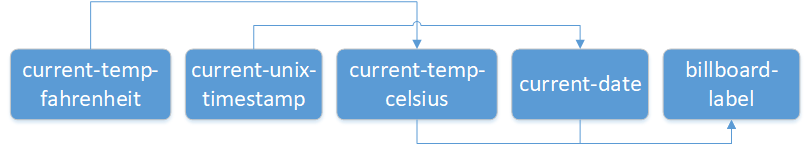
\includegraphics[width=\textwidth]{images/Language-FrDataflow-TopologicallySortedList.png}}
	\caption{The billboard as a topologically sorted list}
	\label{fig:language-frdataflow-topologically-sorted-list}
\end{figure}

\subsubsection{The update loop}

To implement the update behavior, each signal has a boolean flag indicating if it is stale or not. 
Upon startup of the runtime, FrDataFlow initializes a never ending update loop which loops over the topologically sorted list (as shown in figure \ref{fig:language-frdataflow-topologically-sorted-list}), skipping any signals which are not stale. 
If it encounters a stale signal, the lambda function that was provided during the creation of the signal will be called with the latest values of the parent signals. The signal is flagged as no longer being stale, and its direct children are flagged as stale immediately. Take for example an update of the current temperature. We start with a situation where the current date and temperature are already known and shown on the billboard, so the state of the signal graph looks like what is shown in figure \ref{fig:language-frdataflow-1}. 
Note that built in signals (i.e. source signals) in FrDataFlow do not have a staleness flag, because they are kept up to date in separate background loops. For example, a standalone infinite loop keeps the \textit{current-seconds} signal up to date by updating its value every second. 

\begin{figure}[h]
	\centerline{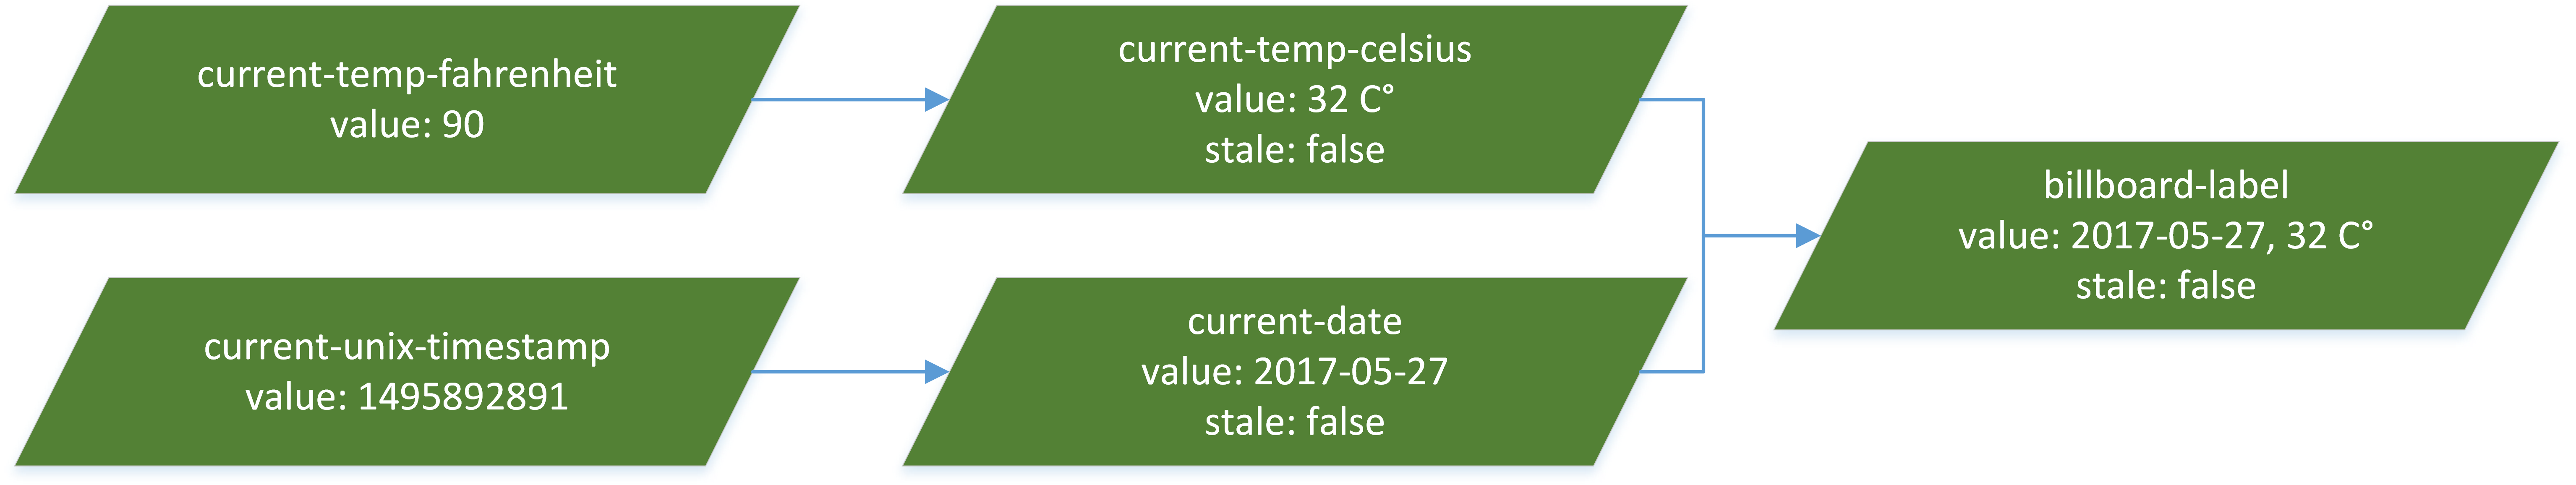
\includegraphics[width=\textwidth]{images/language-frdataflow-1.png}}
	\caption{The initial state of the billboard. \textbf{\textcolor{OliveGreen}{Green = Not stale}}}
	\label{fig:language-frdataflow-1}
\end{figure}

When the new temperature is observed, the direct children of \textit{current-temp-fahrenheit} are flagged as stale, as shown in figure \ref{fig:language-frdataflow-2}.

\begin{figure}[h]
	\centerline{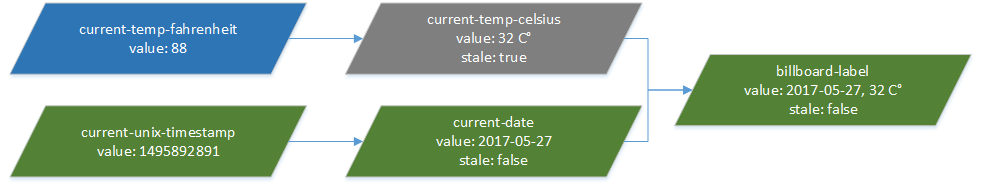
\includegraphics[width=\textwidth]{images/language-frdataflow-2.png}}
	\caption{A new temperature is emitted by current-temp-fahrenheit. \textbf{\textcolor{RoyalBlue}{Blue = New value and not stale}}, \textbf{\textcolor{gray}{Grey = Stale}}}
	\label{fig:language-frdataflow-2}
\end{figure}

The update loop sees that the signal has gone stale, recalculates what its value should be using the value of \textit{current-temp-fahrenheit} and removes the stale flag when its work is done.
However, it also immediately flags \textit{billboard-label} as stale, because it is registered as a child of \textit{current-temp-celsius}, as shown in figure \ref{fig:language-frdataflow-3}.

\begin{figure}[h]
	\centerline{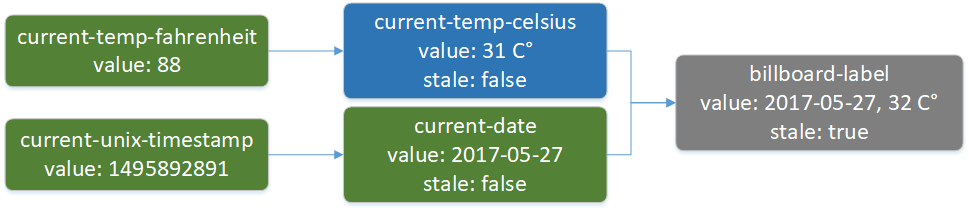
\includegraphics[width=\textwidth]{images/language-frdataflow-3.png}}
	\caption{current-temp-celsius gets recalculated}
	\label{fig:language-frdataflow-3}
\end{figure}

When the update loop moves further down the topologically sorted list, it sees that \textit{billboard-label} is stale now. It grabs the latest values from \textit{current-temp-celsius} and \textit{current-date} and calls the lambda that was used to create \textit{billboard-label}, setting the stale flag to false when it is done. The final result is shown in figure \ref{fig:language-frdataflow-4}. 
At this point, the update loop starts over again, repeating ad infinitum. Every time, the loop checks if a signal is stale and repeats the update process as described above. If no signals are stale, it keeps looping until that changes. 

\begin{figure}[h]
	\centerline{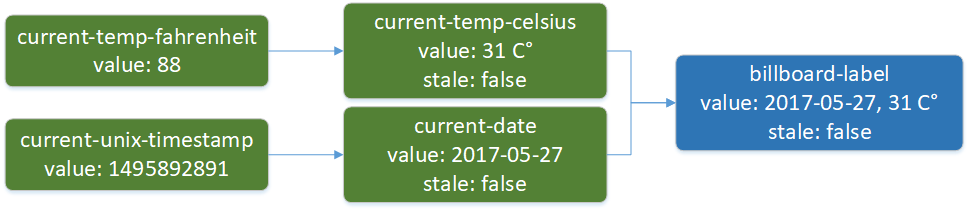
\includegraphics[width=\textwidth]{images/language-frdataflow-4.png}}
	\caption{billboard-label gets recalculated}
	\label{fig:language-frdataflow-4}
\end{figure}

\newpage
\section{Conclusion}

In this chapter the reactive language FrDataFlow was presented with samples and diagrams of its implementation.
It is built as a metacircular evaluator that takes a core subset of the Racket language and extends it with some reactive concepts. FrDataFlow evaluates these expressions in a simulated runtime that forwards statements to the real underlying Racket implementation. 

This language can be used to model reactive data flows and provides a built in update loop to manage the data dependencies between signals. It does this by intelligently looping over the signals while being aware of the dependencies between them. New signals can be created by deriving from other signals and a lift function which produces a single value based on the values of the parent signals.
\chapter{DataFlow Engine}

\section{Introduction}

In this chapter, a dataflow engine is presented based on the work detailed in \citet{saey_extensible_2017}.
This engine is designed to support parallel execution of instructions by queuing all arguments to instructions and executing these in a scope agnostic way.
Tagged token dataflow is an extension to the data flow model where tags are used to distinguish the execution context of tokens, i.e. multiple calls to the same instruction with different arguments.
For the purposes of this thesis, a lightweight version of this engine has been implemented in Racket to facilitate the mapping process from FrDataFlow. Furthermore, we implemented a mapping layer that translates reactive signals to data flow instructions. Even though there were some mismatches that needed to be addressed, the mapping was successful. 

\newpage
\section{Architecture}

\subsection{Execution of instructions}

Take for example a sample program which computes the average of two numbers, as shown in listing \ref{lst:engine-architecture-sample}

\begin{lstlisting}[caption={Computing the average of two numbers},captionpos=b,label={lst:engine-architecture-sample},language=FrDataFlow]
(define (average x y)
  (/ (+ x y) 2))
  
(average 2 6)
(average 1 5)
\end{lstlisting}

This program computes the average of two numbers twice using different arguments. When this program gets evaluated in the data flow engine, the four arguments are added to the token queue, containing information about which execution context they belong to and what should happen to the result. 
In this example, the 2 and 6 belong to the same execution context, while 1 and 5 will belong to a different one. 

\begin{figure}[h!]
	\includegraphics[width=\textwidth]{images/Engine-Architecture-1.png}
	\caption{The \textit{average} instruction gets called twice}
	\label{fig:engine-architecture-1}
\end{figure}

In figure \ref{fig:engine-architecture-1} we see the arguments queued up against the \textit{average} instruction. Colors indicate the execution context, being positioned lower and more to the left indicates their position in the token queue. At this point, the token queue consists of 2, 6, 1 and 5, wrapped in meta data. 

\begin{figure}[h!]
	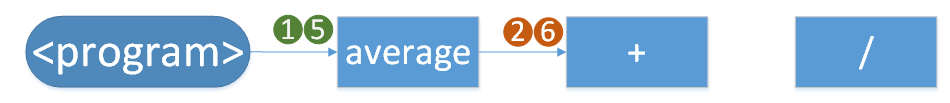
\includegraphics[width=\textwidth]{images/Engine-Architecture-2.png}
	\caption{The arguments are forwarded to the \textit{plus} instruction}
	\label{fig:engine-architecture-2}
\end{figure}

\begin{figure}[h!]
	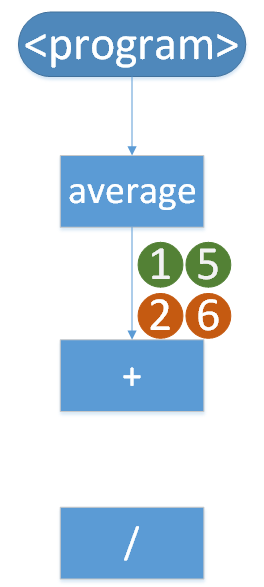
\includegraphics[width=\textwidth]{images/Engine-Architecture-3.png}
	\caption{The next set of arguments are also forwarded to the \textit{plus} instruction}
	\label{fig:engine-architecture-3}
\end{figure}

Since all arguments are present for the first invocation, the \textit{average} instruction gets invoked, as shown in figure \ref{fig:engine-architecture-2}. This calls the plus instruction internally, which adds two new tokens to the queue: 2 and 6.
Because tokens are enqueued at the end, the next thing that happens in figure \ref{fig:engine-architecture-3} is the same step for 1 and 5. Note that tokens are processed one by one, which is not directly obvious from the diagrams. For brevity, the diagrams only show states when an instruction can be executed in the next loop.

\begin{figure}[h!]
	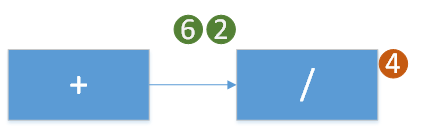
\includegraphics[width=\textwidth]{images/Engine-Architecture-4.png}
	\caption{Results of the \textit{plus} instruction are passed on the \textit{quotient} instruction}
	\label{fig:engine-architecture-4}
\end{figure} 

\begin{figure}[h!]
	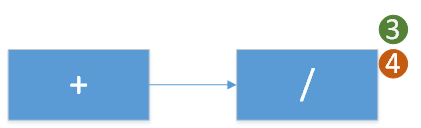
\includegraphics[width=\textwidth]{images/Engine-Architecture-5.png}
	\caption{Results of the second invocation of \textit{plus} are passed on the \textit{quotient} instruction}
	\label{fig:engine-architecture-5}
\end{figure}

When the \textit{plus} instruction has completed its work, it enqueues the result as a new token again, sending it along to the \textit{quotient} instruction. This is possible because of the information contained in the tokens: they know where to go next when instructions have completed. 
In figure \ref{fig:engine-architecture-4} and \ref{fig:engine-architecture-5} we see this process happening for both execution contexts.
Note that the tags are very important here, otherwise the engine would not be aware which arguments belong to the same invocation. There is no guarantee that tokens will always be enqueued in the correct order.

\begin{figure}[h!]
	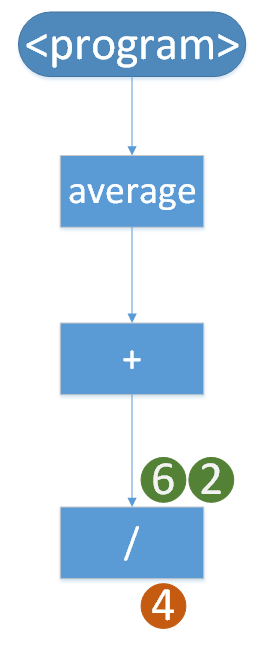
\includegraphics[width=\textwidth]{images/Engine-Architecture-6.png}
	\caption{These results are fed into the quotient operator}
	\label{fig:engine-architecture-6}
\end{figure}

\begin{figure}[h!]
	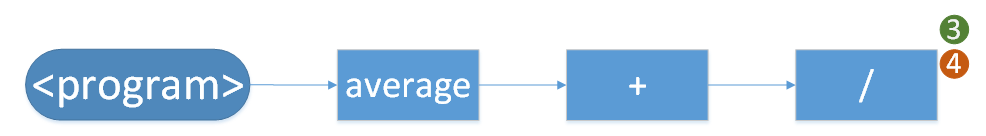
\includegraphics[width=\textwidth]{images/Engine-Architecture-7.png}
	\caption{The second set of results are fed into the quotient operator}
	\label{fig:engine-architecture-7}
\end{figure}

In the end, when the \textit{quotient} instruction has also completed, its results are pushed into the token queue again, as shown by figure \ref{fig:engine-architecture-6} and \ref{fig:engine-architecture-7}. This allows further processing of the data, but is outside the scope of this example. 

To summarize, the general algorithm of the dataflow engine is to process tokens in the queue (FIFO), execute instructions whenever an execution context has all the necessary arguments present and re-enqueue the results of those instructions. Separate invocations are distinguished using tags that denote the execution context.

\section{Mapping of reactive signals to dataflow engine}

To execute our reactive signals on the dataflow engine, a translation step was required to simulate the update loop using the described mechanisms in the dataflow engine.
When we represent reactive programming as a graph, the nodes are signals while the vertices denote dependencies between them.
In the dataflow model, the nodes are instructions and the vertices are data being passed in to them. Therefore, our mapping layers creates data flow nodes for every signal, where the arguments passed in are the parent signal values. When a new value is produced, a token is generated for every child that is subscribed to it.

Taking our example from the Language chapter, we have the following reactive program in figure \ref{fig:engine-mapping-1}.

\begin{figure}[h!]
	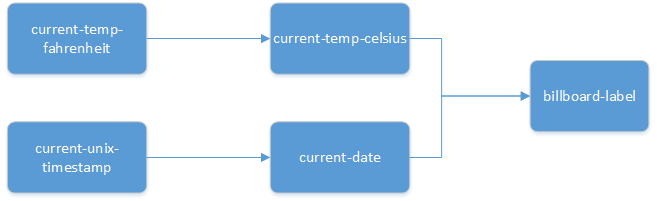
\includegraphics[width=\textwidth]{images/Engine-Mapping-1.png}
	\caption{The billboard program, but the signals are now data flow nodes}
	\label{fig:engine-mapping-1}
\end{figure}

This program behaves exactly the same as the reactive version, the only difference being that is now running atop a dataflow engine.

\subsection{Problems encountered}

\subsubsection{The consumption of arguments in the data flow model}

\paragraph{Problem description}

In reactive programs, signals with a dependency to two or more parent signals are updated whenever at least one of their parents emits a new value. This boils down to the signal functioning as a mapping of the latest values of its parents. Taking our example, this means that when the current temperature changes, the billboard will update immediately, even if the current date has not changed at all.
Similarly, the billboard label updates when the date changes, even if the temperature has not emitted a new value.

In the dataflow engine, an instruction that gets executed consumes its tokens. This is problematic, because when the current temperature emits a new value, it now produces a new token on the queue. 
The billboard label node receives this token, but will keep waiting until the current date produces another token as well. This means that a signal does not update until ALL of its parents have emitted new values.
This was the biggest mismatch between reactive programming and the data flow model, and a perfect solution was not found.

\paragraph{Solution description}

To simulate the same behavior as reactive signals in the data flow model, we had to figure out a way to retrieve the latest values of other parent signals when a new token arrives. 
Although each signal has references to all of its parents, it was not advisable to just read out the latest values and generate extra tokens for the other parents as well. 
This would break our potential for parallelism, because it should be presumed that these dataflow nodes live on and get executed in separate processes and even machines.
The whole premise of the data flow model is that nodes cannot be allowed to access outside state apart from the incoming arguments from the tokens.

The only option that remained was therefore to simulate new signal emissions for all the source signals (signals without parents that get updated by the runtime outside the update loop) whenever one of the source signals emits. Since there is no language support for filtering, throttling or dynamically manipulating the flow of data through the graph, it can be safely assumed that emitting new values from the source signals will ripple through the entire graph, causing all nodes to be updated in the same order. In practice, this meant that whenever a new temperature is sent out, the current second also pushes a value out at the same time. This means the necessary tokens are put on the queue at the same time, simulating the behavior we originally wanted: whenever one parent emits, the other parents do too.

\subsubsection{The evaluation of all instructions in the data flow model}

\paragraph{Problem description}

The data flow engine is actually designed to execute all instructions found in the code, from the highest level abstractions to the lowest primitive operators. The mapping engine was originally designed this way to completely translate not only the signals, but also the statements found in their callbacks to data flow nodes. This meant complete buy-in into the dataflow model, in the hopes of achieving maximum parallelism. However, there is a large mismatch between the traditional Racket language and the dataflow engine: returning values. Whenever a procedure is executed in Racket, it must return a value. In the data flow model, this concept does not exist. Output from instructions is simply enqueued and is not accessible outside the dataflow runtime. Secondly, procedures in Racket carry around with them lexically scoped environments, allowing the use of closures to capture variables or other state that is not enclosed in the body of the procedure definition. 
Again, this violated the core principles of the dataflow engine, which meant we had to scale down the extent to which we made use of the dataflow engine. 

\paragraph{Solution description}

Instead of completely buying into the dataflow engine, we only used its model to implement our reactive signal graph. When parents emit their values, a callback is executed for the signal to update its value. This callback is actually executed inside the interpreter, using the lexical scope assigned to the procedure, without any knowledge or awareness of its presence inside the dataflow engine.
While this has the downside of reduced parallelism, it does improve correctness. Of course, it's impossible to prevent mutating global state or generally causing side effects in these callbacks, but a foolproof mechanism was not the intent of this experiment. 

\section{Conclusion}

In this chapter, we presented a tagged token dataflow engine. This is a runtime that enqueues arguments to instructions and executes these in parallel. 
When interpreting code in the FrDataFlow language, the reactive signals are mapped to dataflow nodes in the engine using a custom mapping layer. During this process, mismatches between reactive programming and the dataflow model are tackled. For example, all source signals emit new values whenever one of them has a new value, to avoid signals waiting in the dataflow engine for inputs from all their parents. Secondly, since return values are not supported in the dataflow engine, the decision was made to only model signals as dataflow instructions and leave the rest of the code execution inside the original interpreter code. 
In the end, we have a reactive system running atop a parallel dataflow engine, triggering updates in the correct way whenever a parent signal emits. 






\chapter{Evaluation}

\section{Introduction}

In this chapter, we investigate the performance characteristics of the two runtimes we created for FrDataFlow. We will explore different types of reactive programs and how they behave under high loads of data, comparing them on a few metrics. More specifically, we will focus on the following metrics:

\begin{description}[style=nextline]
  \item [Latency]		The time it takes for a value to propagate through the entire graph of signals
  \item [Throughput]	The amount of values that can propagate through the entire graph within a certain time frame.
  \item [Scaling]		The amount of performance that can be gained by executing the program in parallel
\end{description}

These objective measurements can provide us with meaningful insight as to how efficient both interpreters are, and what the effects of parallelization are for our benchmarks.

\newpage
\section{Topologies}

Before we can start running benchmarks, we must first define the types of programs that we are interested in profiling. In \textit{Optimizing Distributed REScala} \cite{drechsler_optimizing_2014}, three topologies are suggested that sufficiently represent any reactive program for the purposes of evaluating performance.

\subsection{Linear}

This model is the simplest one: we have a graph of signals where each signal only has one parent and one child. When the source signal emits a new value, it simply propagates through the graph in one linear motion and stops at the end. 

\begin{figure}[h]
	\centerline{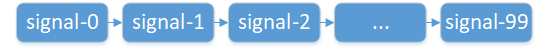
\includegraphics[scale=0.7]{images/Evaluation-Topologies-Linear.png}}
	\caption{A linear topology: each signal has one parent and one child}
	\label{fig:evaluation-topologies-linear}
\end{figure}

\subsection{Fan out}

In this topology, our graph immediately splits up into many children, as shown in figure \ref{fig:evaluation-topologies-fanout}. This is a scenario where one source signal provides important data that every other signal depends upon. The interesting effect of this is when that specific source signal emits a new value, it will trigger an immediate high load of updates for all of its children. 

\begin{figure}[h]
	\centerline{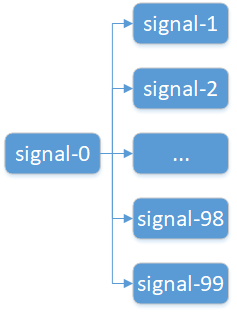
\includegraphics[scale=0.7]{images/Evaluation-Topologies-Fanout.png}}
	\caption{A fan-out topology: one signal with a large amount of children}
	\label{fig:evaluation-topologies-fanout}
\end{figure}

\subsection{Square}

The square topology is expected to be the most common, it provides a signal graph that is not extremely deep such as the linear topology nor is it very wide like the fan-out variant. In this topology, signals have a variable amount of parents and children, shaping the graph into a square. For the purposes of our benchmarks, we will use an exact square graph for simplicity.  

\begin{figure}[h]
	\centerline{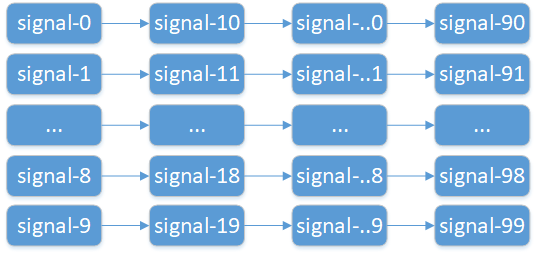
\includegraphics[scale=0.7]{images/Evaluation-Topologies-Square.png}}
	\caption{A square topology: The signal graph is equally deep as it is wide}
	\label{fig:evaluation-topologies-square}
\end{figure}

\section{Benchmarks}

All of the benchmarks in this chapter are run in the Racket VM with unlimited memory (16 GB RAM physical limit) and on an AMD Phenom II X4 955 processor (Quad core, 3.2 GHz). Three sample programs were created with around 100 signals each, each of which implementing one of the three topologies as shown in the diagrams. These programs were each executed three times for 60 seconds, taking the averages of the output to produce the charts in this chapter.
A single source signal was emulated to emit 10 million values per second and the output nodes of the signal graphs were inspected to collect information on how many values were propagate through the graph and at what rate the update mechanisms could keep up with the stream of incoming data. 

\newpage
\subsection{Without dataflow engine}

We will first evaluate the runtime that implements an update loop in the interpreter itself and does not use the dataflow model to keep its graphs up to date. These are the tests for our first runtime for FrDataFlow. 

\subsubsection{Latency}

\begin{figure}[h]
	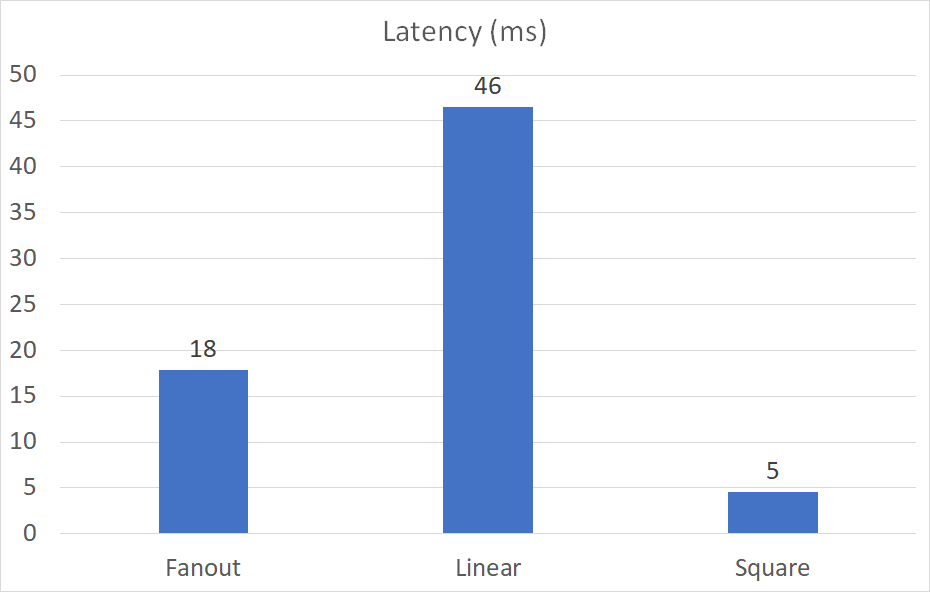
\includegraphics[width=\textwidth]{images/Evaluation-WithoutDataFlow-Latency.png}
	\caption{The latency of signals in FrDataFlow without the dataflow engine}
	\label{fig:evaluation-withoutdataflow-latency}
\end{figure}

Inspecting these results, we conclude that the linear graph show the highest latency, which is expectable: values in this topology travel the longest path of signals before they reach the end. On average, it took nearly 50 ms for a value to propagate from the source signal to the last output node.
More interestingly, values in the fanout topology seem to take longer on average to reach the end than in the square variant. This is counterintuitive, because every value in the fanout graph only needs to pass two signal nodes before it reaches the end. Since the fanout graph contains 99 output nodes and the square graph only 10, it would seem that this gives the square graph a slight edge: these 10 output nodes have to wait less long to be given the chance to announce their output. 

\subsubsection{Throughput}

\begin{figure}[h]
	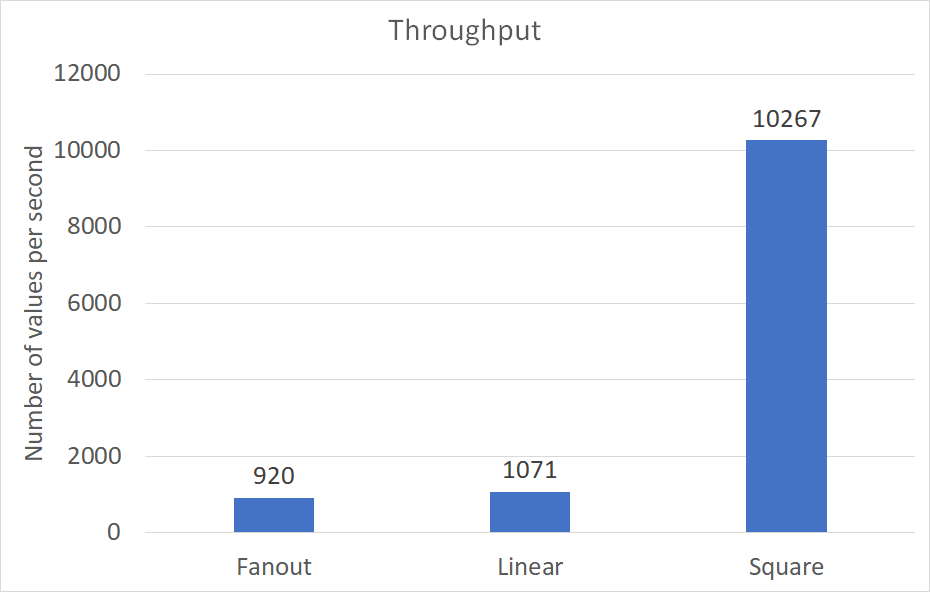
\includegraphics[width=\textwidth]{images/Evaluation-WithoutDataFlow-Throughput.png}
	\caption{The throughput of signals in FrDataFlow without the dataflow engine}
	\label{fig:evaluation-withoutdataflow-throughput}
\end{figure}

Even more so than with latency, the square topology is the clear winner when it comes to the sheer amount of values it can push through the graph per second. The square graph can push out more than 10 000 values per second and is an order of magnitude more efficient compared to the fanout or linear approach, who only managed to process 1 000 values by and large. This makes sense, because every update loop iterates over all the signal nodes once. In the square topology, this means it can propagate 10 values to the end in one loop. The linear version on the other hand can only process one, because when the iteration is happening it is really pushing forward one value from the first signal all the way to the last. Similarly, the fanout approach results in one loop pushing a single value from the first signal to all other signals. The square topology, by splitting up the graph in 10 linear parts, essentially 
parallelizes this work. 

\section{With dataflow engine, single core}

In this section, we repeat the same tests of the previous section but this time using the runtime that sits atop the dataflow engine. The programs are exactly the same, but they are now compiled to dataflow instructions and invoked there. These are the tests for our second runtime for FrDataFlow. 

\subsection{Latency}

\begin{figure}[h]
    \includegraphics[width=\textwidth]{images/Evaluation-WithDataFlow-Latency.png}
	\caption{The latency of signals in FrDataFlow with the dataflow engine}
	\label{fig:evaluation-withdataflow-latency}
\end{figure}

The first thing that is immediately obvious is the increase in latency. While the relative proportions remain the same (the square topology is slightly better than fanout, while the linear topology is clearly the worst in this regard) we observe an average of 50 ms extra latency because we now translate to dataflow instructions. This was to be expected: the use of a dataflow engine brings with it some extra overhead such as the management of the token queue. While 50 ms is considerable, it is not a show stopping performance penalty and is thus acceptable for the gains that can be made in other spaces.

\subsection{Throughput}

\begin{figure}[h]
	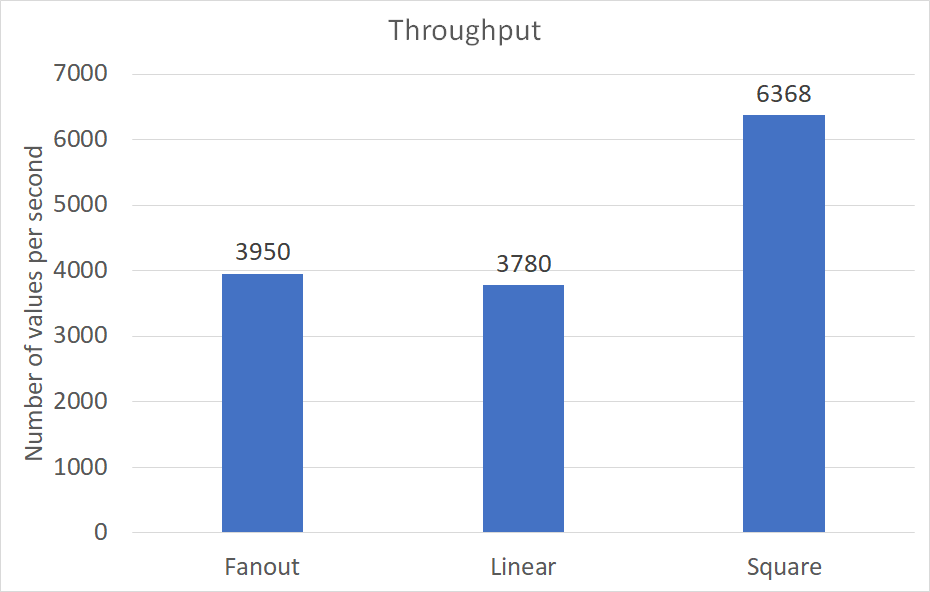
\includegraphics[width=\textwidth]{images/Evaluation-WithDataFlow-Throughput.png}
	\caption{The throughput of signals in FrDataFlow with the dataflow engine}
	\label{fig:evaluation-withdataflow-throughput}
\end{figure}

We observe that the general throughput using the dataflow engine is more efficient than the first runtime. 
Especially the fanout and linear approaches benefit here and see a tripling of their output. The square topology on the other hand is less advantaged by the second runtime and takes a small hit in throughput compared to the first runtime.

The major reason for this increase in throughput can be attributed to the compilation step of the signals that happens in the mapping algorithm. In the first runtime, the update lambdas associated with each signal are fed into the metacircular evaluator which has to lookup variables in the lexical scope and generally introduces a significant overhead just to call a lambda and pass on a value. When running atop the dataflow engine, these update lambdas are fed natively to the dataflow engine which has no knowledge of the metacircular evaluator, which allows it to skip most of the evaluation steps that are necessary in the first runtime.

The reason why the square topology does a little worse is because the update loop in the first runtime is - by accident - ideally optimized for square topologies, while the dataflow engine is not: tokens are just processed one by one, which levels the playing field for all three topologies. 

\subsection{With parallelization}

\section{Conclusion}




\chapter{Future work and limitations}

\section{Introduction}

In this chapter we present the limitations and possible improvements of FrDataFlow. 
The current implementation is rather limited in its functionality because we wanted to focus on the mapping layer and the possibilities of parallelization using the dataflow engine.
However, multiple improvements can still be made. The setup of signals is still a rigid system in that it does not allow the dynamic creation of new signals, the filtering of values or just generally manipulating the timing of value propagation. Every signal always has to emit a value for every set of incoming values. While this already allows for a rich set of programs, these manipulations would be necessary to implement any non trivial program using FrDataFlow. 

\section{Dynamically creating signals}

One of the common patterns in reactive programming is the dynamic creation of new signals based on some state or external input.
In a web environment, imagine a program that searches a database while the user types keywords. This stream of text can be represented as a signal that is attached to the text input field and emits strings upon every keystroke. Then we create a child signal which subscribes which takes these strings and launches an XMLHTTPRequest (ajax request) to fetch the data that satisfies these keywords. Every request again can be modeled as a signal which emits the data that is retrieved and then goes silent. Essentially what this program is doing is dynamically creating a new signal (XMLHTTPRequest) for every value in another signal (the keystrokes). To take this example even further, when the user types another character, we would like to discard any previously created XMLHTTPRequests because we no longer care for their results. Ideally, some sort of cancellation could happen if it is not already too late, but we definitely want to ignore any data that is retrieved based on outdated keywords. This means our dynamically added signals are not only quickly created, but also discarded.

An implementation of this pattern can be observed in the RxJs\footnote{In RxJs, a signal is known as an \textit{observable}. When signals dynamically produce more signals, they are called \textit{higher order observables}.} library. \citep{noauthor_observable_2017}. It contains the \textit{switch} operator, which is visually represented by figure \ref{fig:futurework-dynamicsignals-switch}.

\begin{figure}[h!]
	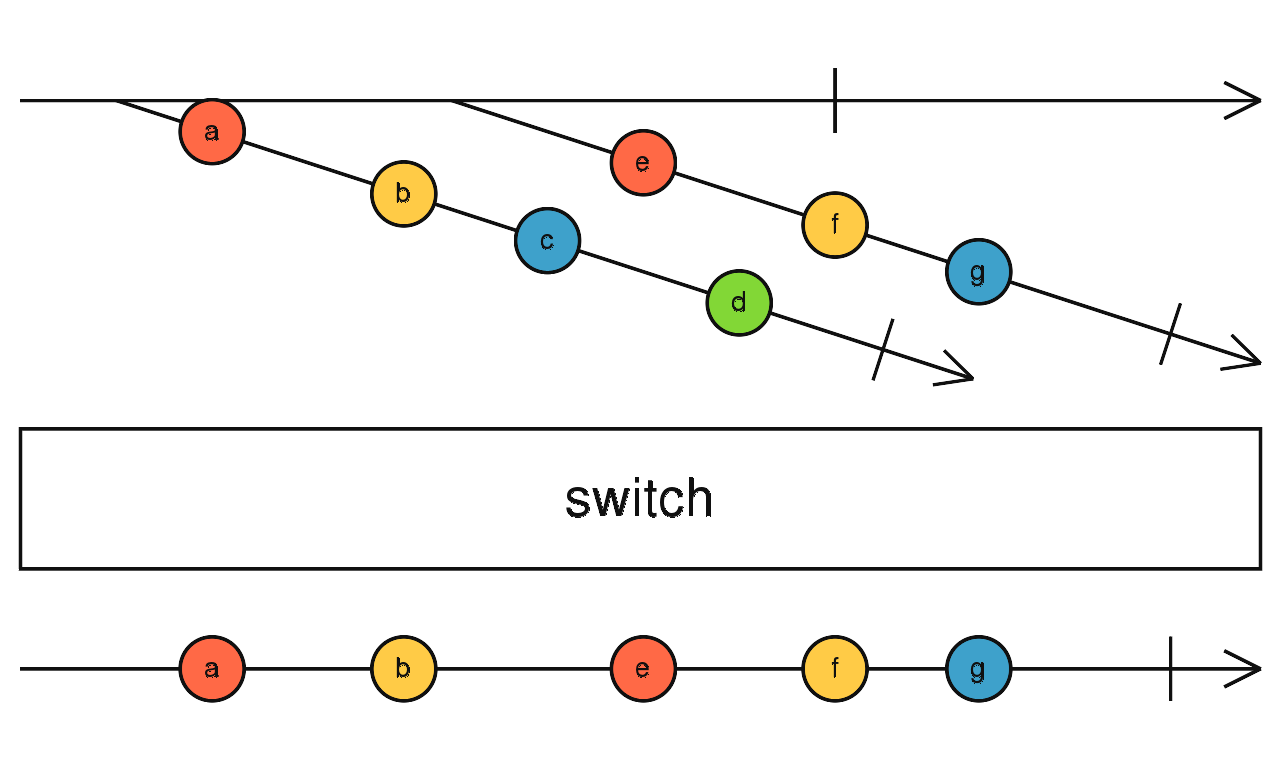
\includegraphics[width=\textwidth]{images/FutureWork-DynamicSignals-Switch.png}
	\caption{A timeline diagram of the \textit{switch} operator in RxJs}
	\label{fig:futurework-dynamicsignals-switch}
\end{figure}

In this figure, we can see a top horizontal arrow which represents the root signal. Values of this signal are transformed into child signals, which on their part can again emit multiple values. 
Since we are only interested in the latest data, we essentially \textit{unsubscribe} from the first child signal when a new value appears in the root signal, so that the sample values c and d never propagate to the end result. 

In the current version of FrDataFlow, it is unfortunately not possible to create new signals at runtime. A possible improvement would be to allow this, which would mean the signal would have to be added to the topologically sorted signals and be translated to a dataflow node. This would also mean that any existing dataflow nodes upon which this new signal depends would have to be updated to also generate tokens for this new node. Similarly, upon destroying signals, this node and all the references to it would have to be updated.

\subsection{Filtering}

Another common practice is filtering of signals, only letting values through which satisfy a certain predicate. Our current implementation of FrDataFlow models signals as a mapping function which takes a set of inputs and produces a new value for every updated set. Filtering would introduce the possibility of not propagating a value at all if certain criteria are not met. In essence, a signal would no longer provide a lambda that has to return a value, but a lambda that can push values into a type of sink when it wants to. This refactoring would allow for a whole category of powerful constructs, such as taking only the first n values, throttling signals, etc. 

An example visualization of the filter function in RxJs can be seen in figure  \ref{fig:futurework-filtering-filter}. 

\begin{figure}[h!]
	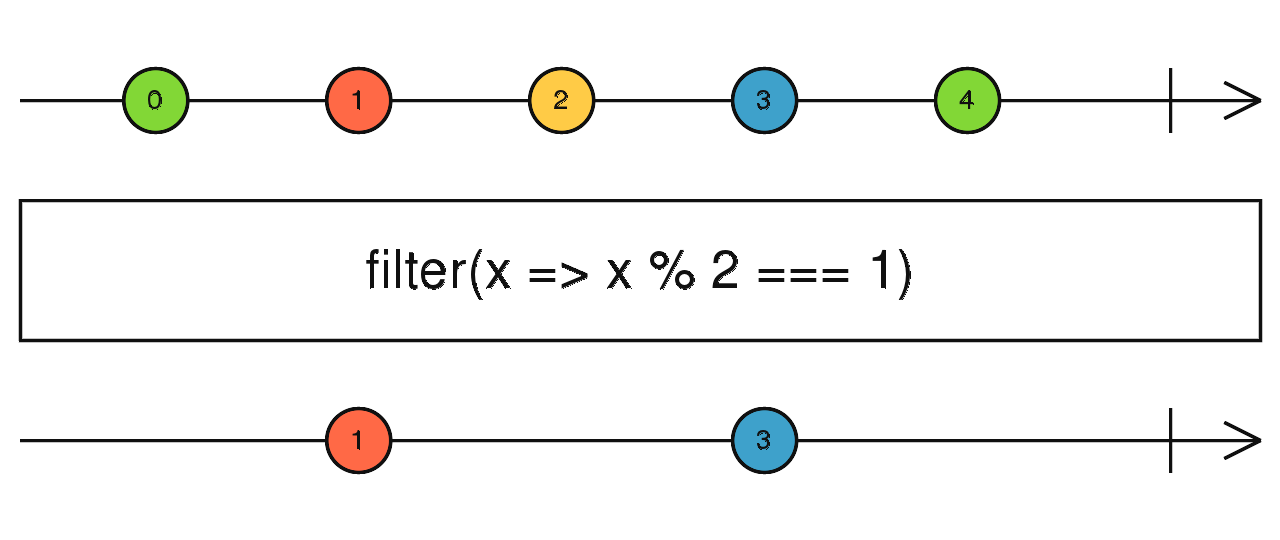
\includegraphics[width=\textwidth]{images/FutureWork-Filtering-Filter.png}
	\caption{A timeline diagram of the \textit{filter} operator in RxJs}
	\label{fig:futurework-filtering-filter}
\end{figure}

We see at the top a signal which produces a stream of numbers. If we create a new signal that filters these numbers using the filter function, we get a new stream of numbers that only contains those that satisfied the predicate. When the number 0 is pushed into the signal lambda, it does not propagate it into the sink of the child signal, which means the value does not go through. 

To implement this pattern in our mapping layer, we would have to ensure that dataflow nodes don't always have to produce new tokens when they are invoked, and a way for nodes to indicate when this should happen or not. However, there is no technical reason why the dataflow engine should not be able to handle this: it is simply the presence of tokens that determines which nodes are invoked, so not emitting these tokens would essentially implement the filtering behavior we have described.


\section{Conclusion}

In this chapter we have shown how FrDataFlow is still a basic language that does not support some powerful concepts such as the dynamic creation of signals or the filtering of values.
If these concepts were to be introduced, they would allow for an implementation of most of the techniques commonly found in other reactive libraries or languages.

This initial version of FrDataFlow has focused mostly on the practical mapping layer from reactive programming to the dataflow model. There are however no immediate technical shortcomings that should prevent us from implementing the modifications presented in this chapter.
\chapter{Related work}

\section{Introduction}

In this chapter, we introduce a few related works and papers that align with concepts described in this dissertation. The language Elm for example describes in detail the challenges of functional reactive programming, tackling many of the same problems and describing similar solutions as encountered in FrDataFlow. Despite the similarities, the difference in platforms (Elm has to adhere to the limitations of the JavaScript execution engine in browsers, while FrDataFlow is constrained to the limits of the Racket runtime) has a significant impact on the potential to parallelization. Another source of inspiration was FrTime, a DrScheme implementation of reactive patterns with some subtle yet powerful differences. Its focus lies more on the implicit transformation of regular programs to reactive programs, while FrDataFlow remains very explicit about the existence of signals.

Finally, we discuss the virtual machine design of the dataflow engine that FrDataFlow uses to execute its instructions. This VM builds on the principles of tagged token dataflow and provides a platform upon which the reactive nodes in FrDataFlow are scheduled and executed. 

\section{Reactive programming}

\subsection{Elm}

In 2012, Evan Czaplicki wrote his dissertation on Elm \citep{czaplicki_elm:_2012}, a functional reactive programming language for the web. In this paper, he presents a new language \textit{Elm} that supports concurrent functional programming for the web. Elm is compiled down to JavaScript using a compiler written in Haskell and promises to produce no runtime errors when everything compiles. 
Most of the reactive programming concepts in FrDataFlow were actually heavily inspired by Elm, such as \textit{signals} and the \textit{lift} function. 
Another concept inspired by Elm is signal graphs: reactive primitives as nodes and value flows as edges. Of course, source signals are a bit different in the web. For example, Elm provides source signals that represent mouse clicks, mouse positions or generally any kind of DOM event which is captured by the standard library. In the isolated, experimental little world of FrDataFlow, primitive source signals other than the current time were hard to come by. 

\subsubsection{Order of events}

Looking at a signal graph, it is easy to imagine the parallel execution of the nodes. However, the order of events is very important. 
Take for example the signal graph shown in figure \ref{fig:relatedwork-elm-eventsorder}.

\begin{figure}[h!]
	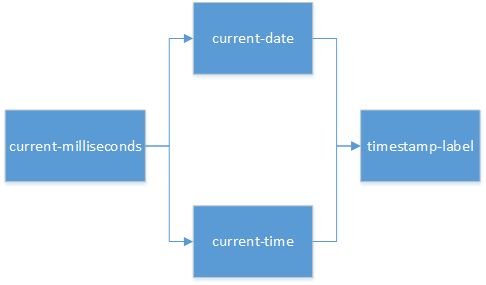
\includegraphics[width=\textwidth]{images/RelatedWork-Elm-EventsOrder.png}
	\caption{The current timestamp is based on two different computations of \textit{current-milliseconds}}
	\label{fig:relatedwork-elm-eventsorder}
\end{figure}

If a new value appears for current-milliseconds (the number of milliseconds since 1 Jan 1970), we compute the current date and current time separately, to combine these two data points into a single label called \textit{timestamp-label}. Imagine now that the computation of the current time takes significantly longer than the computation of the current date. In fact, we can contemplate that the derivation of the time would actually need to derive the date first, and then use the remaining milliseconds from midnight to determine the time. Of course, depending on the date and the timezone, this could result in different clock times.
This leads us to conclude that the calculation of \textit{current-time} is slower than \textit{current-date}. 

Now imagine that these computations are run in parallel and that their outputs are piped to the timestamp label as fast as the hardware allows it. If the date is so much faster to process, it becomes possible that the timestamp label starts receiving more than one \textit{current-date} for every \textit{current-time}, leading to situations where the date and time that are shown do not both trace back to the same value of \textit{current-milliseconds} they were derived from. 

In Elm, this problem was fixed by the introduction of a global event dispatcher, which imposes a few constraints on the signal graph update loop:

\begin{itemize}
	\item Signals with more than one parent must wait for all parents to produce a value before recomputation happens. This is the same approach taken in FrDataFlow. 
	\item When source signals emit a new value, all nodes receive that event and pass forward a "nothing changed" notification. In FrDataFlow, the approach is to simply push the current value. 
\end{itemize}


\subsubsection{Parallelization}

In Elm, the constraints of the platform are slightly different. The JavaScript runtime does not really provide native parallelization\footnote{Web workers exist, which were designed offload work in background threads. However, they come with two rather expensive limitations, the first being that messages between workers must be primitive data types, so there is no support for passing along functions with closures, only simple messages such as strings or numbers. Secondly, these web workers directly map to operating system threads, making them quite expensive to set up and tear down. The end result is that these workers are not a good fit for the small, atomic computations we are dealing with in reactive nodes.}, so while the language itself could perfectly support parallelism, unfortunately its platform does not. 

Elm does provide some workarounds for when the synchronous nature of its node processing causes performance bottlenecks, namely asynchronous updates. This keyword decouples a subset of the graph from the main graph and allows it to update independently, avoiding the situation where it would have to wait for long running synchronous updates. However, this is still purely a data correctness and timing feature and unfortunately does not tackle the lack of parallelization support.

In fact, the paper does mention a possible solution to run Elm programs in parallel: if closures can be avoided somehow (for example by compiling to an intermediate language which explicitly lists the used captured variables) and if functions are passed as strings (and then dynamically interpreted inside the workers), web workers could technically provide a parallel execution mechanism. It was not considered worthwhile though, because of the amount of overhead to orchestrate this and the possible security ramifications.

\subsection{FrTime}

Another project that is closely related to FrDataFlow is \textit{FrTime}. This is a reactive programming language that implicitly implements signals for primitive operators. The idea is that applications written in regular Scheme could be switched over to FrTime to introduce reactive programming without having to rewrite the code. Contrary to FrDataFlow, expressions in FrTime do not require explicit use of the lift operator, but are implicitly used when any of the primitive operators are used. For full effect, FrTime provides a REPL (Read Eval Print Loop) console which takes expressions and immediately prints the result. There is an extra feature though: values which are signals keep getting updated in the history. When for example the plus operator is applied to a fixed number and the current seconds, this creates a signal which continuously updates with the result, inside the console. Rather than evaluating the expression and returning a signal like in FrDataFlow, FrTime immediately returns a value and keeps updating that value, even inside the REPL history. 

\begin{lstlisting}[caption={REPL in FrTime},captionpos=b,label={lst:relatedwork-frtime-repl}]
> seconds 			
1496651429
> (even? seconds) 
#f
> (+ 10 seconds)
1496651439
\end{lstlisting}

See the listings \ref{lst:relatedwork-frtime-repl} and \ref{lst:relatedwork-frtime-repl-5s}. In the first sample, some commands are entered into the REPL and their output is shown below each command.
Note that the listing \ref{lst:relatedwork-frtime-repl-5s} simply shows exactly the same screen from listing \ref{lst:relatedwork-frtime-repl} but 5 seconds later. It is not revealed to the user that the expressions he is using are built with signals that update in the background. It only becomes clear, as time goes by, that these values automatically update in the REPL.

\begin{lstlisting}[caption={REPL in FrTime, 5 seconds later},captionpos=b,label={lst:relatedwork-frtime-repl-5s}]
> seconds
1496651434
> (even? seconds)
#t
> (+ 10 seconds)
1496651444
\end{lstlisting}

\subsubsection{Push-driven evaluation}

A major difference between FrTime and FrDataFlow is its update model. FrDataFlow implements what is called a push driven evaluation. This means that parent signals - or producers, as FrTime calls them - have references to their children (dependents in FrTime). When a parent signal gets updated, it can follow along the edges of its dependencies to ripple the change forward in the graph. Since child signals do not hold references to their parents, closures are used during the signal construction process to capture references to these parents in the callback procedure.

In FrDataFlow, callbacks and closures are not an essential part of the update mechanism. All signals are stored in a topologically sorted graph, where each signal can access its parents and children. When a new value propagates through the graph, the update loop simply grabs the necessary information from the parent signals to provide to the child.

FrTime's callback model in combination with their queue based update algorithm actually comes with a string of performance problems, which they try to address by \textit{lowering} \cite{burchett_lowering:_2007} their operators, essentially collapsing multiple operations into one to reduce overhead and to minimize the graph size. Although this considerably improves execution time, it unfortunately also reduces parallelization opportunities by growing the size of one signal node. In FrDataFlow, no such optimizations are considered. 

\section{Dataflow Model}

\subsection{Virtual machine design for the execution of languages on dataflow machines}

In \cite{saey_extensible_2017}, a virtual machine design is presented to execute instructions on dataflow machines. This VM tries to offer a framework in which the principles of tagged token dataflow are strictly adhered to, while allowing full access to the tokens and execution context from within a single dataflow node, i.e. an operation. This allows the creation of operations which can manipulate the destination they send data to, enabling conditional statements and dynamic flow in general. To enable closures, operations also receive access to the active working memory of the current context. 
In short, this design is intended to support all common flows expected in a high level language, such as function calls, closures, recursion, exception handling, etc.

For FrDataFlow, a minimal version of the engine described has been implemented in Racket, to avoid the overhead of having to communicate between Racket and Python. 

\section{Conclusion}

In this chapter, we presented other research that closely relates to and strongly inspired FrDataFlow. Elm, the web programming language with a strong focus on FRP, introduced many of the same concepts also applied in FrDataFlow. FrTime has similar semantics, but chose to hide its internals more from the end user. For the execution of our signal nodes, we applied the virtual machine design of DVM in Racket to map our reactive nodes as dataflow operations. 






\chapter{Conclusion}

In our research for this dissertation, we explored the initial steps needed to map from reactive programs to the dataflow execution model. 
These steps included creating our own experimental language FrDataFlow, writing a mapping algorithm from a reactive graph to a dataflow graph and executing the latter atop a data flow engine as described in \cite{saey_extensible_2017}. This chapter will revisit the original problems we set out to tackle, the solutions we proposed and conclude with some closing remarks. 

\newpage
\section{Revisiting the problem statement}

Reactive programming is an event-first programming paradigm well suited for reactive systems (e.g. user interfaces, robotics, etc.) that provides the concept of signals which can be composed using declarative operators.
These signals are a common abstraction over I/0, events and asynchronous computations and provide a single interface to model these concepts.
Efficiency and timing is essential to create responsive and reliable reactive systems. However, the majority of reactive programming implementations are not designed to support parallelism, which is necessary to maximally utilise the processing power of modern processors. We propose to run reactive programs atop the dataflow execution model to make maximal use of the parallelization abilities provided by the underlying host. This execution model invokes instructions when the inputs are available and does not provide any form of global state, allowing instructions that do not share data dependencies to be invoked side by side. 

\newpage
\section{Contributions}

We implemented an experimental Racket based language called FrDataFlow that adds reactive concepts to a subset of Racket constructs. This language was implemented using two different interpreters: one which directly implements the reactive mechanism in Racket and serves as a reactive runtime by manually keeping the graph of signals up to date using an update loop, as described in chapter 3 - Language.
The second implementation delegates the responsibility of keeping the reactive graph up to data to a dataflow engine implementation by mapping the signals to dataflow instructions in such a way that the signals behave the same as in a regular reactive system. 

More specifically, we provided the following contributions:

\begin{description}[style=nextline]
	\item[An interpreter for a reactive language] We designed and implemented an interpreter based on FrTime, but which chooses to provide explicit reactive operators rather than implicitly applying reactivity. This interpreter applies a traditional evaluation model to keep signals up to date, in the form of a signal update graph. 
	\item[A mapping algorithm from signals to dataflow instructions] We implemented an algorithm that maps the concepts of reactive programming to instructions in the dataflow execution model and solves a major mismatch between the two: the consumption of arguments in dataflow, as described in Chapter 4. Furthermore, we showed that reactive programs can be correctly translated to dataflow instructions so that they behave exactly the same. 
	\item[Comparison of a traditional reactive evaluation model and signals atop the dataflow execution model] We evaluated the performance of both approaches in terms of latency, throughput and scalability and showed that the platform overhead of parallelism, for now, does not outweigh the benefits of parallelism. We do note however that single threaded dataflow execution already brings with it benefits in terms of throughput, although at the cost of latency.
\end{description}

\newpage
\section{Final remarks}

The ultimate goal of this dissertation was to explore the possibilities of executing reactive programs atop a dataflow engine, in the hopes of achieving highly parallel execution of these programs. 

We notice that high level paradigms such as reactive programming are becoming increasingly popular, but they usually come with a performance cost due to these abstractions. In reaction to this, we tried to address these concerns by proving that the abstractions reactive programming makes can be correctly translated to a horizontally scalable execution model, namely a dataflow engine. In doing so, we touched on an unexplored subject in this space, making a meaningful contribution to both the world of reactive programming and the dataflow execution model. 

We look forward to seeing the further evolution of both in the future and the new insights they bring to the world of software development.  

\newpage
\appendix
\renewcommand{\chaptermark}[1]{\markboth{\MakeUppercase{\appendixname}\ \thechapter.\ #1}{}}
\chapter{Appendix} \label{App:AppendixA}
\addtocontents{toc}{\protect\setcounter{tocdepth}{0}}


\bibliographystyle{apacite}
\bibliography{ThesisBib} % change to your bib!
\end{document}
